\documentclass[10pt]{beamer}
\usepackage{amsmath,amssymb,longtable,hhline}
\usepackage{mathrsfs}
\usepackage{xcolor}
\usepackage{hyperref}
\usepackage{multicol}
\usepackage{anyfontsize}
\usepackage{minted}

\usemintedstyle{tango}
\newcommand{\ltprgsize}{\fontsize{5}{5}\selectfont}
%\newcommand{\ltprgsize}{\footnotesize}
\setminted{fontsize=\footnotesize{},mathescape}

\definecolor{mygreen}{rgb}{0,0.6,0}
\definecolor{mygray}{rgb}{0.5,0.5,0.5}
\definecolor{mymauve}{rgb}{0.58,0,0.82}

\hypersetup{
    bookmarks=true,         % show bookmarks bar?
    unicode=true,           % non-Latin characters in Acrobat’s bookmarks
    pdftoolbar=false,        % show Acrobat’s toolbar?
    pdfmenubar=false,        % show Acrobat’s menu?
    pdffitwindow=false,     % window fit to page when opened
    pdfstartview={FitH},    % fits the width of the page to the window
    pdftitle={Construction techniques of Baikal microbiome research information-computational environment},    % title
    pdfauthor={Evgeny Cherkashin, Alexey Shigarov, Vasily Khristyuk},     % author
    pdfsubject={model driven architecture},   % subject of the document
    pdfnewwindow=true,      % links in new PDF window
    colorlinks=true,       % false: boxed links; true: colored links
    linkcolor=red,          % color of internal links (change box color with linkbordercolor)
    citecolor=green,        % color of links to bibliography
    filecolor=magenta,      % color of file links
    urlcolor=blue           % color of external links
}

\usepackage{pifont}

\usetheme{Warsaw}
\usecolortheme{crane}
%\useinnertheme{rectangles}
%\setbeamertemplate{itemize item}{\scriptsize\hbox{\donotcoloroutermaths\ding{113}}}
\definecolor{darkding}{RGB}{200,56,0}
\setbeamertemplate{itemize item}{\scriptsize\hbox{\color{darkding}{\bfseries\ding{113}}}}
\setbeamertemplate{itemize subitem}{\tiny\raise1.5pt\hbox{\donotcoloroutermaths$\blacktriangleright$}}
\setbeamertemplate{itemize subsubitem}{\tiny\raise1.5pt\hbox{\donotcoloroutermaths$\blacktriangleright$}}
\setbeamertemplate{enumerate item}{\insertenumlabel.}
\setbeamertemplate{enumerate subitem}{\insertenumlabel.\insertsubenumlabel}
\setbeamertemplate{enumerate subsubitem}{\insertenumlabel.\insertsubenumlabel.\insertsubsubenumlabel}
\setbeamertemplate{enumerate mini template}{\insertenumlabel}

\beamertemplatenavigationsymbolsempty

\usepackage{iftex,ifxetex}
\ifPDFTeX
  \usepackage[utf8]{inputenc}
  \usepackage[T1]{fontenc}
  \usepackage[russian]{babel}
  \usepackage{lmodern}
  \usefonttheme{serif}
\else
  \ifluatex
    \usepackage{unicode-math}
    \defaultfontfeatures{Ligatures=TeX,Numbers=OldStyle}
    \setmathfont{Latin Modern Math}
    \setsansfont{Linux Biolinum O}
    \setmonofont{Fira Mono}[Scale=MatchLowercase]
    \usefonttheme{professionalfonts}
    % \setmathfont[
    %     Ligatures=TeX,
    %     Scale=MatchLowercase,
    %     math-style=upright,
    %     vargreek-shape=unicode
    %     ]{euler.otf}
  \fi
\fi

%\useoutertheme{split}
%\useinnertheme{rounded}
\setbeamertemplate{background canvas}[vertical shading][bottom=white!80!cyan!20,top=cyan!10]
%\setbeamertemplate{sidebar canvas left}[horizontal shading][left=white!40!black,right=black]

\graphicspath{{pics/}}

\providecommand{\email}[1]{\texttt{#1}}
\usepackage{changepage}
\newcommand{\GB}[1]{\colorbox{green}{#1}}
\newcommand{\BB}[1]{\colorbox{blue}{#1}}
\newcommand{\RB}[1]{\colorbox{red}{#1}}
\newcommand{\btprgsize}{\fontsize{7}{7}\selectfont}

% --------------------------

% \def\cite#1{(#1)}

\begin{document}

\setbeamertemplate{background canvas}[vertical shading][bottom=white,top=white]
\setbeamercolor{background canvas}{bg=white}

\title{Integration of Geological Data as a Knowledge Graph}
\author[E.~Cherkashin, O.~Lunina, T.~Cherkashina, V.~Pellinen, A.~Gladkov]{\bfseries%
  \underline{Evgeny Cherkashin}, Oksana Lunina,  Tatiana Cherkashina, Vadim Pellinen, Anton Gladkov}
\institute{\normalsize Matrosov Institute for System Dynamics and Control Theory, \\ SB RAS, Irkutsk, Russia\\
  Institute of the Earth’s Crust, SB RAS, Irkutsk, Russia
  \\[1em]
\email{\href{mailto:eugeneai@icc.ru}{eugeneai@icc.ru}}%
}
\date[2021]{
IWCI--2021, Baikalsk, Russia
}
%\date{\today}
\maketitle

\begin{frame}
  \frametitle{Problem statement}
  Integration the collected geological data so they can be
  \begin{itemize}
  \item easily accessed
  \item of a standardized representation
  \item integrated with the data sources of the similar structure (access way and data representation paradigm) % e.g. DBPedia.org LOD
  \item thus, reuse the existing data sources for the domain modeling
  \item processed within Big Data paradigm
  \item represented as cartographical work (map) dynamically with/without need of GIS software installation
  \end{itemize}
  The requested requirements are fulfilled with the present Semantic Web technologies.
\end{frame}

\begin{frame}[fragile]
  \frametitle{Semantic web technologies \& Knowledge graphs}
  Semantic Web (WEB 3.0) is characterized with
  \begin{itemize}
  \item Technological basis, oriented to the web % User applications are always comprises of interconnected distributed web-services.
  \item Standardized data formats, storage, and processing
  \item Open principles of data publishing
  % \item Knowledge Graph (KG) construction techniques
  \item Services for data storage and access provision
  \item Generalized and special user interfaces are used for data presentation\vspace{1em}
  \end{itemize}
%\end{frame}

% Knowledge graphs changed the aspects to the knowledge base as being a part of whole totality of knowledge, implying the obeying the global standards and techniques of its acquisition and processing.

%\begin{frame}
%  \frametitle{Knowledge Graphs}
For the Knowledge Graphs (KG), the following is of interest.
 \begin{itemize}
  \item Converged notions \textbf{data} and \textbf{knowledge} as something is \textbf{known}
  \item Contain data, relations, and metadata (vocabularies)
  \item Distinguished \textbf{node filling in} and \textbf{processing} graph triples, \emph{e.g.}, withing SPARQL queries with UPDATEs
  \item Allow \textbf{postpone} the formal definition of a schema
  \item Three types of graph schemata: \textbf{semantic} (aimed at generalization), \textbf{validating} (\textbf{e.g.} semantics, \textbf{completeness} w.r.t. sets of relations), and \textbf{emergent} (infer a set of generalized structures and re-represent the KG).
  \end{itemize}
\end{frame}


\def\textbfr#1{\textbf{{\color{red}#1*}}}

\begin{frame}
  \frametitle{Linked Open Data (LOD) star evaluation}
  Data are available in
  \begin{itemize}
  \item[\textbfr{1}] any format \textbf{openly}
  \item[\textbfr{2}] a \textbf{structured format}, such as Microsoft Excel file format (.xls)
  \item[\textbfr{3}] a \textbf{non-proprietary structured format}, such as .csv
  \item[\textbfr{4}] \textbf{W3C standards}, like using RDF and employing URIs
  \item[\textbfr{5}] a hypercontent form \textbf{having links to other Linked Open Data sources}
  \end{itemize}
  \begin{flushright}
   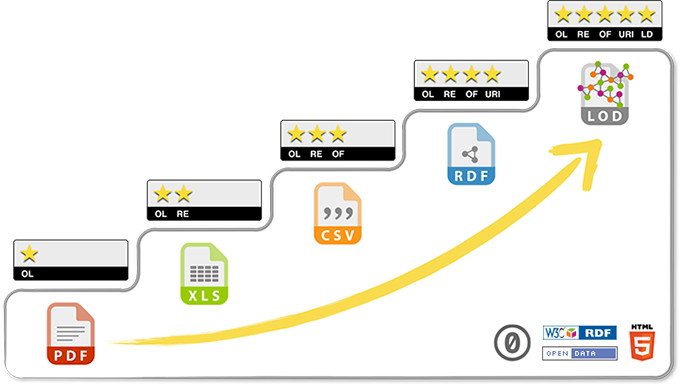
\includegraphics[width=0.7\linewidth]{5-star-lod.png}
  \end{flushright}
\end{frame}

\begin{frame}
  \frametitle{The Aim and the plan}
  The \textbf{aim of the project} is to represent geological data accumulated at IEC SB RAS and other institutes into the Semantic Web infrastructure.
  \begin{itemize}
  \item Design a web-based GIS system, representing data from SPARQL endpoints
  \item Convert the existing data into RDF adhering LOD
  \item Implement natural language query interface using GeoBase (\copyright~Borland) with a conversion into a SPARQL query
  \item Bidirectional versioned data transfer between user GIS (QGIS, OSM Mapnik) and the SW storage % The reason of the usage of OSM Mapmik is the various already implemented data processing service, e.g., GPS traces as raw material for modeling the map.
  \item Implement various analytical functionality for domain problem solving
  \end{itemize}
\end{frame}

% \begin{frame}
%   \frametitle{}
%   \centering
%   \includegraphics[width=\linewidth]{microbiome-study.png}
% \end{frame}

\begin{frame}
  \frametitle{Related works: LinkedGeoData project}
  The project \cite{lgd} was aimed at representing OpenSteetMap (OSM) data as a Knowledge Graph (KG).
  \begin{itemize}
  \item Resembles the DBPedia project formalizing Wikipedia data but on the OSM;
  \item Converts SM data into RDF adhering LOD;
  \item Designed and ontology for object georeferencing (nodes);
  \item Relation of the object to DBpedia, GeoNames, icon sets;
  \item Taxonomy of the objects on a various levels (Road \to Way (list of nodes)); % and Fig 3 of the LGD paper.
  \item Stated the relations between nodes and ways defining complex objects;
  \item REST and SPARQL (does not work now) for actual data;
  \item Live updates from OSM changesets.
  \end{itemize}

\end{frame}

% Namespaces
% lgd: http://linkedgeodata.org/triplify/
% lgdo: http://linkedgeodata.org/ontology/
% wgs84: http://www.w3.org/2003/01/geo/wgs84_pos#
% fao: http://www.fao.org/countryprofiles/geoinfo/geopolitical/resource/
% dbpedia: http://dbpedia.org/resource/
% rdf: http://www.w3.org/1999/02/22-rdf-syntax-ns#
% rdfs: http://www.w3.org/2000/01/rdf-schema#
% owl: http://www.w3.org/2002/07/owl#
% xsd: http://www.w3.org/2001/XMLSchema#
% georss: http://www.georss.org/georss/

\begin{frame}
  \frametitle{Related works: LinkedGeoData project}
  % Figures of Ontology and
  % usage examples
\end{frame}

\begin{frame}[fragile]
  \frametitle{Related Works: GeoLink Knowledge graph}
  GeolLinkk KG \cite{geolink}
  \begin{itemize}
  \item includes diverse information as port calls made by oceanographic cruises, physical sample metadata, research project funding and staffing, and authorship of technical reports;
  \item implements LOD (4 of 5 stars) and federated SPARQL integration;
  \item contains 45 millions RDF triples with ontologies and geo-visualization tools;
  % \item describes interlinked \textbf{R2R}, expeditions, \textbf{BCO-DMO}, oceanography, \textbf{IODP}, ocean floor microbiome, \textbf{MBLWHOI}, marine life papers, \textbf{SESAR}, rock samples, \textbf{DataONE}, metadata of external research,  \textbf{AGU-NSF}, projects \and conferences, \textbf{NGDB}, sediment geochemy, \textbf{USAP}, Antarctica ice.
  \end{itemize}
  In the project, an update procedure (harvesting) is implemented to ensure the consistence of the KG w.r.t. the geo-base ontology (GBO).
\end{frame}

\begin{frame}
  \frametitle{Related Works: GeoLink Knowledge graph}
  % Example image from \cite{geolink}
  The GeoLink knowledge graph is deployed at \url{http://data.geolink.org}.
\end{frame}


% The reference \cite{iwaniak} contains a good review of KG GIS activities related to spacial semantic data representation,  importing, crossreferencing and entity relation techniques and tools development.

\begin{frame}
  \frametitle{Related Works: Integrating LOD into GIS}
  The project \cite{abid} deals with developing a web GIS automatically publishing DBPedia data.
  \begin{itemize}
  \item LOD resembles Open Government Data principles
  \item Modules are
    \begin{itemize}
    \item GIS is Google Map API v3
    \item SPARQL used to query DBPedia
    \item Viewing DBPedia data with Data Table plug-in of JQuery
    \end{itemize}
  \item
  \item Test application allows user querying celebrities by their home town/city pointed by mous on the Google Map.
  \end{itemize}
\end{frame}

\begin{frame}
  \frametitle{Related Works: Integrating LOD into GIS}
  % Figure of GIS and SPARQL query
\end{frame}


\begin{frame}
  \frametitle{Related Works: Publishing Geodata LOD in context dependent pages}
  The project \cite{iwaniak17} goal is to convert existing GIS data into explicit knowledge, thus, forming a Spatial Data Infrastructure (SDI).
  \begin{itemize}
  \item Integrate existing geoportal data into a KB, including dynamic data
  \item Geoportal data must be LOD, e.g., HTML is enriched with RDFa
  \item Relation interpreters implemented as Expert systems (``building near forest'')
  \item Semantic enrichment of raw data to make it more usable/discoverable
  \item Targeting to GeoSPARQL (sfIntersects, sfOverlaps, sfTouches, sfWithin, sfContains))
  \item Metadata inference from the data source properties
  \item Test application is to integrate public services data in Mazowieckie Voivodeship of Poland, queries are realized by a limited set of keywords
  \end{itemize}
\end{frame}

\begin{frame}
  \frametitle{Related Works: Publishing Geodata LOD in context dependent pages}
  % figure 1 of Concept of system architecture
  % figure 2 HTML example
\end{frame}


\begin{frame}
  \frametitle{Resources to be presented: Active faults of the South of
    East Siberia}
   % Screenshot of the system
\end{frame}

\begin{frame}
  \frametitle{Resources to be presented: Active faults of the South of
    East Siberia}
  The fault data have the following properties:
  \begin{itemize}
  \item Faults are the objects having linear projection on the surface, and a depth and a slope in the lithosphere;
  \item Various geological events are also subjects of presentation.
  \item Any object accompanied with various valued characteristics having also characteristics, e.g., unit name, measurement precision and related publications.
  \item Images, tables, expedition trails are a also used as auxiliary materials.
  \end{itemize}
\end{frame}

\begin{frame}
  \frametitle{Resources to be presented:  Contamination of  Olkhon Island}
   % Generate a map from the existing data
\end{frame}

\begin{frame}
  \frametitle{System architecture}
  \centering
  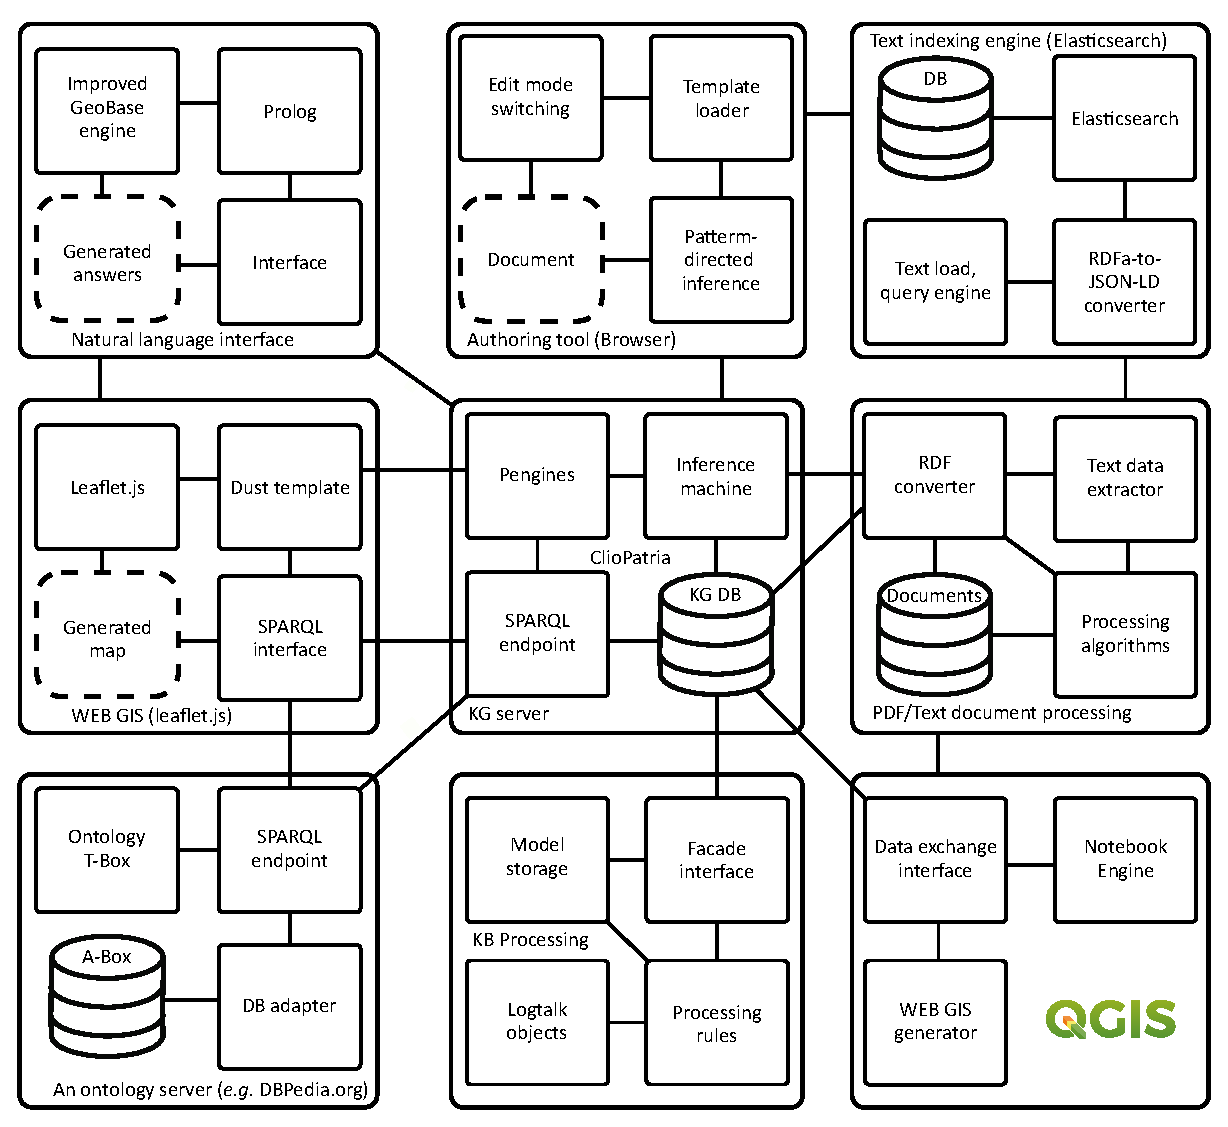
\includegraphics[width=0.8\linewidth]{architecture.pdf}
\end{frame}

\begin{frame}
  \frametitle{Conclusion}
  [[[]]]The following results have been obtained as for today:
  \begin{itemize}
  \item Biologists' activities are mastered, investigated and regular patterns are described.
  \item A technique for interpretation of Mothur interfaces has been developed, implemented, refined and extended.
  \item Transformation tools are tested in application areas and no significant technical problems were detected.
  \item A technique of document authoring is being developed and adapted to the domain.
  \item Integration with Galaxy project is the primary aim of the future development.
  \end{itemize}
  The source codes are available at \url{https://github.com/isu-enterprise/icc.xmitransform}, \url{https://github.com/eugeneai/icc.mothurpim}.

  This research is supported by Irkutsk scientific center of SB RAS, project No 4.2;
\end{frame}

\begin{frame}
  \frametitle{External links}
  \begin{columns}
    \begin{column}{0.5\textwidth}\centering
      % \includegraphics[width=1\linewidth]{qrcode-pdf.eps}
      The presentation URL
    \end{column}
  \end{columns}
\end{frame}

\begin{frame}
  \begin{center}
  \Large Thanks for Your interest in our project!
\end{center}
\end{frame}

\begin{frame}
  \begin{center}
  \Large Auxiliary materials
\end{center}
\end{frame}

\begin{frame}
  \frametitle{Technologies used (open source)}
  Python-3.x.x (\url{http://python.org}),\\
  ZCA (\url{https://muthukadan.net/docs/zca.html}),\\
  SWIG (\url{http://swig.org/}),\\
  SWI-Prolog (\url{https://www.swi-prolog.org/}),\\
  Logtalk (\url{https://logtalk.org/}),\\
  ClioPatria (\url{https://cliopatria.swi-prolog.org/home}),\\
  Pengines (\url{https://pengines.swi-prolog.org/docs/index.html}),\\
  LOV (\url{https://lov.linkeddata.es/dataset/lov/}),\\
  Elastic Search (\url{https://www.elastic.co/}),\\
  Kyotocabinet (\url{https://fallabs.com/kyotocabinet/}),\\
  DBPedia (\url{https://wiki.dbpedia.org/}),\\
  Mothur (\url{https://mothur.org/}),\\
  Galaxy (\url{https://usegalaxy.org/}),\\
  R (\url{https://www.r-project.org/}), \\
  Dust.js (\url{https://akdubya.github.io/dustjs/})
\end{frame}\begin{frame}
  \frametitle{Technologies used (open source)}
  Python-3.x.x (\url{http://python.org}),\\
  ZCA (\url{https://muthukadan.net/docs/zca.html}),\\
  SWIG (\url{http://swig.org/}),\\
  SWI-Prolog (\url{https://www.swi-prolog.org/}),\\
  Logtalk (\url{https://logtalk.org/}),\\
  ClioPatria (\url{https://cliopatria.swi-prolog.org/home}),\\
  Pengines (\url{https://pengines.swi-prolog.org/docs/index.html}),\\
  LOV (\url{https://lov.linkeddata.es/dataset/lov/}),\\
  Elastic Search (\url{https://www.elastic.co/}),\\
  Kyotocabinet (\url{https://fallabs.com/kyotocabinet/}),\\
  DBPedia (\url{https://wiki.dbpedia.org/}),\\
  Mothur (\url{https://mothur.org/}),\\
  Galaxy (\url{https://usegalaxy.org/}),\\
  R (\url{https://www.r-project.org/}), \\
  Dust.js (\url{https://akdubya.github.io/dustjs/})
\end{frame}



\begin{frame}[fragile]
  \frametitle{Semantic Web technologies in representation of models
    during transformation}
  \begin{itemize}
  \item Assimilates experience of domain basic researches trending to standardization;
  \item Regular set of triples denote a graph (T-Box, A-Box);
  \item Standard vocabularies are formally described (\verb|rdfs:domain|, \verb|rdfs:range|);
  \item Supported with most programming systems (libraries, inference engines, SPARQL);
  \item RDF has a way of global element identification, \emph{i.e.} we can refer the same object from different software systems;
  \item SWI-Prolog supports direct queries to a graph, as well as interpreting some predicates (\verb|rdfs:label|, \verb|dc:title|), wraps sparse RDF structure into a predicate arguments; ontological server ClioPatria;
  \item There is simple way of data security implementation (\verb|rdfs:seeAlso|);
  \item By means of Semantic Web \& LOD we are able to organize data transfer between heterogeneous information systems.
  \end{itemize}
\end{frame}

\begin{frame}
  \frametitle{Used ontologies}

  Standardized ontologies

  \begin{itemize}
  \item Friend-of-a-friend (\textbf{foaf}) for agent information: individuals, legal entities, program agents.
  \item Provenance (\textbf{prov}) for making references between documents.
  \item Dublin Core (\textbf{dc}) for published resource metadata mark up.
  \item DBPedia resource (\textbf{dbr}) to refer external classes and instance objects.
  \item Schema.org (\textbf{schema}) for Google, Yandex, Yahoo, \emph{etc}. searchable objects, structural elements.
  \item The Bibliographic Ontology (\textbf{bibo}) used for literature reference mark up.
  \item Open annotation (\texttt{oa}) as an ``bookmark'' ontology.
  \end{itemize}

  Non-standard ontologies

  \begin{itemize}
  \item Ontology \texttt{nssp} for Mothur source code processing results.
  \item Ontology \texttt{uml} for XMI representation.
  \end{itemize}
\end{frame}

\begin{frame}
  \frametitle{Document authoring and storage}
  In most cases documents are created as a result of
  \begin{itemize}
  \item creative activity of a person with a text processors (authoring);
  \item printing a digital copy or a data record in a database;
  \item aggregation operation over database records (report).
  \end{itemize}
  Then it is stored either as a physical paper and/or a digital document (PDF, DOCX, HTML).

  Since 2000-th, Semantic Web and Linked Open Data (LOD) is being developed, allowing
  \begin{itemize}
  \item structural storage of data within published documents;
  \item processing stored data computationally;
  \item integration of data structures and data objects globally.
  \end{itemize}

  The \textbf{aim of this research} is to develop technologies, software and services allowing construction of digital archives supporting document data inclusion and inference from existing documents.
\end{frame}

\begin{frame}
  \frametitle{Open Annotation (oa)}
\begin{adjustwidth}{-3em}{-3em}
  \centering
  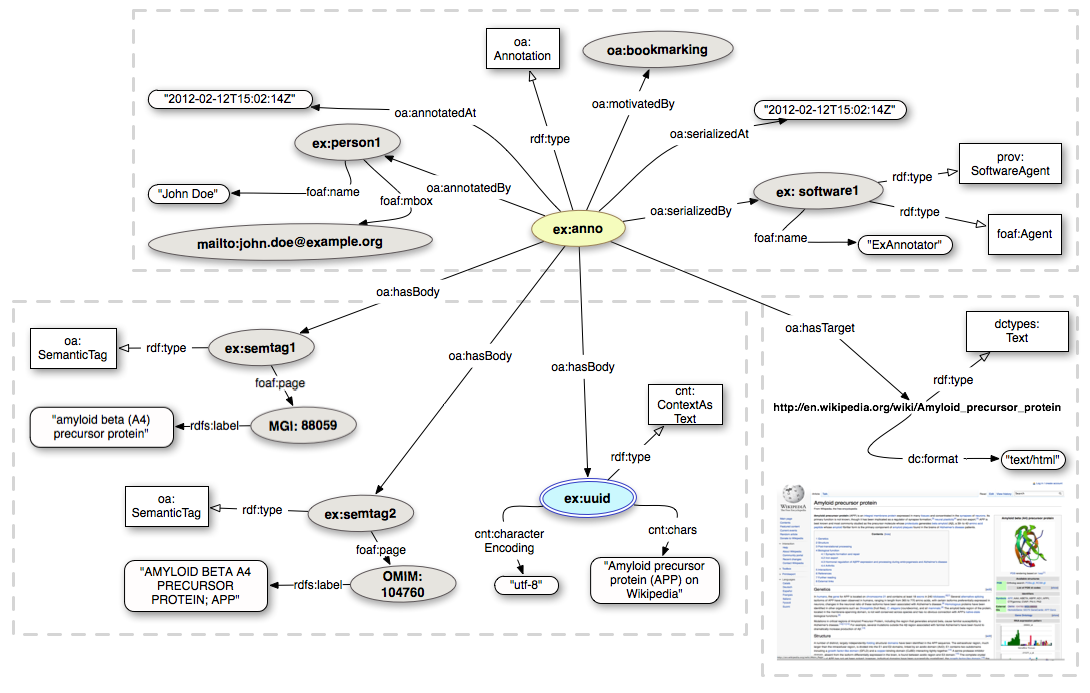
\includegraphics[width=1\linewidth]{Open-Annotation_CB_Bookmarking_and_Semantically_Tagging_A_webpage_spec20130128.png}
\end{adjustwidth}

\end{frame}

\begin{frame}[fragile,fragile]
  \frametitle{Representation}
  % \begin{block}{}
  %   \textbf{Целью} исследования является создание методики разработки процедур трансформации (PD\footnote{Platform [description] model.}) в виде ОО-модулей.
  % \end{block}
  % \begin{columns}
  %   \begin{column}{0.5\linewidth}
  %     % \includegraphics[width=1\linewidth]{pics/scenario-ru-wo-mothur.pdf}
  %   \end{column}
  %   \begin{column}{0.6\linewidth}
  %     Задачи исследования:
  %     \begin{itemize}
  %     \item Изучить синтаксические структуры Logtalk в аспекте структурирования знаний;
  %     \item Предложить методику представления трансформации в виде ОО-модулей;
  %     \item Реализовать библиотеку объектов и классов для МДА;
  %     \item Тестирование библиотеки на примере.
  %     \end{itemize}
  %   \end{column}
  % \end{columns}

\begin{adjustwidth}{-1.5em}{-1.5em}
\begin{minted}[escapeinside=||,fontsize=\btprgsize]{xml}
<html lang="ru" xmlns=http://www.w3.org/1999/xhtml
|\GB{xmlns:taa}|=http://irnok.net/engine/rdfa-manipulation
xml:lang="ru" metal:define-macro="page">
<head> . . . . </head>
<body prefix="rdf: http://www.w3.org/1999/...-ns# foaf: http://xmlns.com/foaf/...
imei: imei.html# course: https://irnok.net/college/plan/01..16-...\
%D0\%BA_PB-SM.plm.xml.xlsx-....2.3.1.html#"  resource="#post"
typeof="schema:CreativeWork sioc:Post prov:Entity">
<!-- The application control panel -->

<main lang="ru" resource="#annotation" typeof="oa:Annotation" id="main-doc-cnt">
<div property="oa:hasTarget" resource="#course-work-prog"></div>
<article property="oa:hasBody" typeof="foaf:Document curr:WorkingProgram"
         resource="#course-work-program" id="main-document">
  <div |\GB{taa:content}|="imei:title-page"></div>
  <div |\GB{taa:content}|="imei:neg-UMK"></div>
  <section id="TOC" class="break-after"> <h2>Table of Contents</h2>
    <div id="tableOfContents"></div>
  </section>
  <section id="course-description" resource="#description"
           property="schema:hasPart" typeof="schema:CreativeWork">
    <div property="schema:hasPart" resource="#purpose"
         typeof="dc:Text cnt:ContentAsText" >
      <div property="cnt:chars" datatype="xsd:string">
        <h2 property="dc:title" datatype="xsd:string">
           Aims and objectives of the discipline (module)</h2>
        <p>The aim of teaching the discipline ...</p>
      </div>
   </div>
  . . . . . . . .
\end{minted}
\end{adjustwidth}
\end{frame}

\begin{frame}
  \frametitle{Linked Open Data, LOD}
  \begin{enumerate}
  \item Information is published in Internet with open access license;
  \item It is represented in a machine-readable form, e.g., Excel table instead of a bitmap picture;
  \item An open format used, e.g., CSV instead of Excel;
  \item The format is based on W3C recommended standards, allowing RDF and SPARQL reference;
  \item Published data refer to objects, forming context.
  \end{enumerate}
  Thus, applications publish data as relations of objects (entities).
\end{frame}

\begin{frame}
  \frametitle{Logtalk as transformation definition language}
  We have chosen Logtalk as it
  \begin{itemize}
  \item inherits widely known Prolog language syntax and runtime;
  \item implemented as macro package, performance penalties are about 1.5\%;
  \item has flexible semantics: we can define transformations and constraints within the same syntax;
  \item implement object-oriented knowledge (rules) structuring, encapsulation and replacement;
  \item compositional way of transformation implementation;
  \item powerful engine to post constraints on object-to-object messages (events);
  \item has implementation for many Prolog engines.
  \end{itemize}
  The <<regular>> language allow us to use its libraries not directly related to MDA transformations.
\end{frame}


\begin{thebibliography}{99}
\bibitem{b1}

\bibitem{hogan}
  AIDAN HOGAN, EVA BLOMQVIST, MICHAEL COCHEZ, CLAUDIA D’AMATO, et al Knowledge Graphs.
  \url{https://arxiv.org/abs/2003.02320v5}
\end{thebibliography}


\end{document}

%%% Local Variables:
%%% mode: latex
%%% TeX-master: t
%%% End:
